\documentclass[aps,prl,twocolumn,tightenlines,superscriptaddress,showpacs]{revtex4-1}
\usepackage{epsfig,rotating,amsmath,lineno}
\usepackage{multirow}
\usepackage{subcaption,graphicx}




\begin{document}

\title{Electromagnetic properties of the isotones with $  N=50  $ with the p35-i3 Hamiltonian}

\author{J. A. Purcell}
\affiliation{Department of Physics and Astronomy, Michigan State University, East Lansing, Michigan 
48824-1321,
USA
and Facility for Rare Isotope Beams, Michigan State University, East Lansing, Michigan 48824-1321,
USA}
\author{B. A. Brown}
\affiliation{Department of Physics and Astronomy, Michigan State University, East Lansing, Michigan 
48824-1321,
USA
and Facility for Rare Isotope Beams, Michigan State University, East Lansing, Michigan 48824-1321,
USA}




\begin{abstract}



\end{abstract}

\maketitle

\section{Introduction}

The properties of the isotones with with $  N=50  $ have historically been testing ground for
shell-model configuration interaction (CI) calculations.

We consider the electromagnetic data for low-lying states of nuclei between $^{78}$Ni and $^{100}$Sn
that can be described by protons in $  ({0f_{5/2}, 1p_{3/2}, 1p_{1/2}, 0g_{9/2}}  $
(the $  \pi j4  $ model space).
The region between $^{90}$Zr and $^{100}$Sn is well established territory where many
wavefunctions are dominated by $  (1p_{1/2}, 0g_{9/2})  $ orbitals
\cite{talmi60}, \cite{cohen64}, \cite{aurbach65}, \cite{vervier66}, \cite{ball72}, 
\cite{gloeckner73}, \cite{blomqvist85}.
The full $  \pi j4  $  space has been considered previously with Hamiltonians derived
with the singular-valued decomposition method (SVD)
\cite{jun45}, \cite{jw88}, \cite{jj44a}, as well as those obtained VS-IMSRG methods \cite{Yuan24}.
This paper is based on set of  newly derived SVD Hamiltonians called p30-i3, p35-i2 and p35-i3 
\cite{p35i3}.
In the notation px-iy, x stands for the number of SVD parameters and y stands for
the ab-initio starting points used in \cite{p35i3}.

The starting point for the Hamiltonians in derived in \cite{p35i3}
are those obtained with the  VS-IMSRG method. These are
obtained using the EM 1.8/2.0 NN$+$3N interaction \cite{Heb2011} in a
harmonic oscillator basis with frequency $  \hbar \omega=12  $ MeV,
truncated to 13 major shells ($  2n+l \leq  $ $  e_{\rm max}=12  $). We normal order
with respect to the Hartree-Fock ground state of the reference and discard the
residual 3N interaction. We then decouple the $  \pi j4  $ valence space,
using the Magnus formulation of the IMSRG.
The results obtained with the standard approximation \cite{sr19}, truncating all
operators at the two-body level throughout the flow, including inside
nested commutators are labeled IMSRG(2) in \cite{p35i3}.
The Hamiltnoians obtained
with the SVD method starting with IMSRG(2) are are labeled $  i2  $.

Another starting point labeled IMSRG(3f2) in \cite{p35i3}
introduces a correction in which intermediate three-body operators arising
in nested commutators are incorporated by rewriting the double
commutator in a factorized form while maintaining the same computational
scaling as the IMSRG(2) approximation \cite{He24}. As in ref. \cite{He24}, we include factorized 
terms
with a one-body intermediate during the flow, and include terms with a
two-body intermediate at the end of the flow. We perform the procedure for
two different references, $^{78}$Ni and $^{100}$Sn, corresponding to empty
and full valence spaces, respectively, and take the average of the two resulting
valence space Hamiltonians as our starting point for the fitting procedure.
The Hamiltnoians obtained
with the SVD method with starting with IMSRG(3f2) are are labeled $  i3  $.

We showed in \cite{p35i3} that the IMSRG(3f2) provided a better starting
point for describing the experimental energy data in the sense that
the rms deviation obtained with $  p<10  $ SVD parameters was
much smaller with IMSRG(3f2) compared to IMSRG(2). Thus,
IMSRG(3f2) might provide a better input for the linear combinations
of $  69-p  $ SVD parameters that are not well determined from experimental
data.


In \cite{p35i3} we showed that the optimal number number of SVD parameters
was about $  p=35  $ based on the minimum in the rms deviations in trial sets of data.
For the purpose of investigating the Hamiltonian uncertainties
in the observables we also obtained a Hamiltonian with $  p=30  $
SVD parameters.


\section{Electromagnetic observables}









One can express the one-body reduced matrix element for the $  n  $-particle wave
function in the form of a product over one-body transition densities
(OBTD) times reduced single-particle matrix elements (SPME)
$  <k_{\alpha }||O^{\lambda }||k_{\beta }>  $
$$
<f||\hat{O}^{\lambda }||i>\, =  <n \omega _{f} J_{f}||\hat{O}^{\lambda }||n \omega _{i} J_{i}>
$$
$$
= \displaystyle\sum _{k_{\alpha } k_{\beta }} {\rm OBTD}(f i k_{\alpha } k_{\beta } \lambda )
 <k_{\alpha }||O^{\lambda }||k_{\beta }>,       \eqno({1})
$$
where the OBTD is given by
$$
{\rm OBTD}(f i k_{\alpha } k_{\beta } \lambda )
= { <n \omega _{f} J_{f}||[a^{+}_{k_{\alpha }}\otimes \tilde{a}_{k_{\beta }}]^{\lambda }||n \omega 
_{i} J_{i}>
\over  \sqrt{ (2\lambda +1)}   }.       \eqno({2})
$$
The labels $  i  $ and $  f  $ are a shorthand notation for the initial
and final state quantum numbers $  (n \omega _{f} J_{f})  $ and $  (n \omega _{i} J_{i})  $,
respectively.
The $  k_{\alpha }  $ label the spherical single-particle states
$  (n,\ell ,j)  $ used in the model space.
The NuShellX code \cite{nushellx} provides the wavefunctions and the
resulting OBTD.

The $  <k_{\alpha }||O^{\lambda }||k_{\beta }>  $ are the SPME
obtained with the $  E\lambda   $ and $  M\lambda   $ operators.
We consider magnetic moments
$$
\mu  = \sqrt{\frac{4\pi }{3}}   <i,J,M=J\mid {\hat O}(M1)\mid i,J,M=J>
$$
$$
= \sqrt{\frac{4\pi }{3}}
 {\left( \begin{array}{ccc} J & 1 & J \\ -J & 0 & J \end{array}\right) }
<i,J||{\hat O}(M1)||i,J>,       \eqno({3})
$$
quadrupole moments
$$
Q = \sqrt{\frac{16\pi }{5}}   <J,M=J\mid {\hat O}(E2)\mid J,M=J>
$$
$$
= \sqrt{\frac{16\pi }{5}}
 {\left( \begin{array}{ccc} J & 2 & J \\ -J & 0 & J \end{array}\right) }
<i,J||{\hat O}(E2)||i,J>,       \eqno({4})
$$
and reduced transition probabilities
$$
B(O^{\lambda },i \rightarrow f) = \frac{\mid <f||\hat{O}^{\lambda }||i>\mid ^{2}}{2J_{i}+1}       
\eqno({5})
$$



We consider mainly the B(M1) and B(E2) with the
standard form of the SPME as given in \cite{jw88em}.
B(E1) are zero since the parity-changing $\lambda$=1 operator
does not connect any of the orbitals in the  $  j4  $ model space.
B(M2) are not considered since the parity-changing $\lambda$=2 operator
it limited to only one, $  0g_{9/2}-1f_{5/2}  $,
of the 10  SPME with one orbital in the $  j4  $ model
space involved in M2 transitions.
We have a short section on B(E3) as observed in inelastic scattering
experiment.

For $  M1  $ the SPME involve spin and orbital g-factors which
are usually treated as effective parameters to take into account
configuration mixing outside the $  j44  $ model space
and mesonic-exchange currents. We use the
orbital-dependent effective g-factors
obtained from fits to data in \cite{jw88em}.
For $  E2  $ the SPME involve radial integrals.
It is common to harmonic-oscillator radial wavefunctions.
For example,  a value of $  b^{2}=4.481  $ for the oscillator parameter
was used in \cite{jw88em}.
In addition, one uses an effective proton charge $  e_{p}  $
to take into account mixing with configurations
that are not included in the $  j4  $ model space.
In \cite{jw88em} a value of $  e_{p}=2.0  $ was needed with
their harmonic-oscillator radial wavefunction assumption.
It is better to use more realistic nucleus-dependent
radial wavefunctions obtained with energy-density functionals (EDF).
For this purpose we use the Skx Skyrme functional \cite{skx}.
With this EDF a value of $  e_{p}=1.8  $ gives a good
reproduction of  all of the $  E2  $ data we consider (see Sec. ?).


\section{Uncertainties related to the choice of Hamiltonian}

Here we compare global sets of electromagnetic observables obtained with the
new p35-i3, p35-i3 and p30-i3 Hamiltonians together with
older Hamiltonians, jun45 \cite{jun45}, and jj44a \cite{jj44a}.
The purpose is to use these comparisons to deduce Hamiltonian uncertainties
in the observables. We note that all of these Hamiltonians are
based on fits to data in the $  \pi j4  $ model space, except
for jun45 which is based on a fit to data in larger
proton-neutron $  jj44  $ model space.

We calculated observables for all nuclei between $^{80}$Zn
and $^{98}$Cd and divided for results into those for nuclei with $  A < 88  $
and those for nuclei with $  A \geq 88  $. The
wavefunctions for low-lying states with $  A<88  $ are dominated
by the three orbitals $  (0f_{5/2},1p_{3/2},1p_{1/2}  $
and those with  $  A \geq 88  $ are dominated by
the two orbitals $  (1p_{1/2},0g_{9/2})  $. It was found
in \cite{p35i3} that rms deviation between experiment
and theory for the binding energies excitation
energies was significantly larger in the first group (0.12 MeV).
than those in the second groop (0.05 MeV). Thus,
we can anticipate that the rms deviations in the
various observables will be larger in the first
group compared to the those in the second group.

For each Hamiltonian we calculated the magnetic and quadrupole
moments for the first state of each $  J^{\pi }  $.
Also we calculated the B(M1) and B(E2) for the first state
of each $  J^{\pi }  $ with the first state $  (J+2)^{\pi }  $
We did not include those for which the states were less
that 200 keV from the second state with the same $  J^{\pi }  $.
For set of each set of comparisons we give the rms differences
in the specific observables. These values are
indicative of the associated theoretical uncertainties.

We show the comparison of results obtained with the IMSRG(3f2)
starting Hamiltonian for two different values of the
number of VLC linear combinations varied (30 and 35) in
Figs. 1 and 2. As expected the rms difference is
always larger for nuclei $  A<88  $ compared to those
for $  A \geq 88  $. For the moments (Fig. 1)
and B(E2) (Fig. 2-cd)
this difference is about a factor of two. For the
B(M1) the difference is much larger. The reason
is that the small B(M1) (WU = 1.79 $\mu_{N}^{2}$) arise from
cancellations between components in Eq. (1)
which  are particularly sensitive to small
changes in the Hamiltonian.

We find a particular outlier for the B(E2)
in Fig. 2c with (p30-i3,p35-i3) values of (4,142) e$^{2}$ fm$^{4}$.
This comes from the 7/2$_{1}^{-}$ to 3/2$_{1}^{-}$ transition in
$^{81}$Ga. As seen in Fig. 9 of \cite{p35i3}, there
are two low-lying 3/2$^{-}$ states in $^{81}$Ga.
The B(E2) for the 7/2$_{1}^{-}$ to 3/2$_{2}^{-}$ transition
are (74,8) e$^{2}$ fm$^{4}$. It is not clear what part
of the Hamiltonian is responsible for the
interchange of properties for these B(E2) transitions.

The calculated gamma-decay branching of the 7/2$^{-}$
state to the (3/2$^{-}_{1}$,5/2$^{-}_{1}$) states is (25,75)\%
for p35i3 and (1,99)\% for p30i3.
The gamma-decay data of \cite{ga81} gives
(0,100)\% for the state at 1.40 MeV. Assuming
this is the 7/2$^{-}$ state, the data is in agreement
with the p30i3 Hamiltonian result.






We show the comparison of results obtained with the
IMSRG(2)and IMSRG(3f2)
starting Hamiltonian for 35 varied VLC linear combinations,
(p35-i2) and (p35-i3), respectively in Figs. 3 and 4.
The scatter and rms deviations are similar to
the (p30-i2) and (p35-i3) comparisons discussed above.

The jj44a Hamiltonian \cite{jj44a} was obtained from a
fit to the $  N=50  $ energy data as known in the year 2004.
The comparison of electromagnetic results
obtained with jj44a and p35-i3 are shown in Fig. 5 and 6.
The scatter is significantly worse compared to the
previous comparisons, particularly for the B(M1) and
B(E2) in Fig. 6.

Finally, in Figs. 7 and 8 we show the comparison
of the electromagnetic results obtained with the
jun45 Hamiltonian compared to p35-i3.
The scatter is much worse. This reflects the
fact that the jun45 Hamiltonian was obtained from
a much wider set of nuclei. In particular,
the $  T=1  $ part of  the jun45 Hamiltonian is influenced
by data for the nickel isotopes.
In \cite{jj44a} differences in the $  T=1  $ Hamiltonians
obtained from the $  N=50  $ isotones and the $  Z=28  $
isotopes were discussed. In particular, the
relatively lower energy
of 2$^{ + }$ states in $^{70-78}$Ni compared to those in $^{92}$Mo-$^{98}$Cd
results in the inversion of seniority two and four
states in $^{72-76}$Ni compared to $^{94}$Mo-$^{96}$Cd.
Thus, one concludes that "universal-type" Hamiltonians
are useful, but one can do better with local Hamiltonians
designed from a specific range of nuclei. Ultimately
one should consider and construct nucleus-dependent
Hamiltonians in the spirit of VS-IMSRG calculations \cite{sr19}.
























\begin{figure}
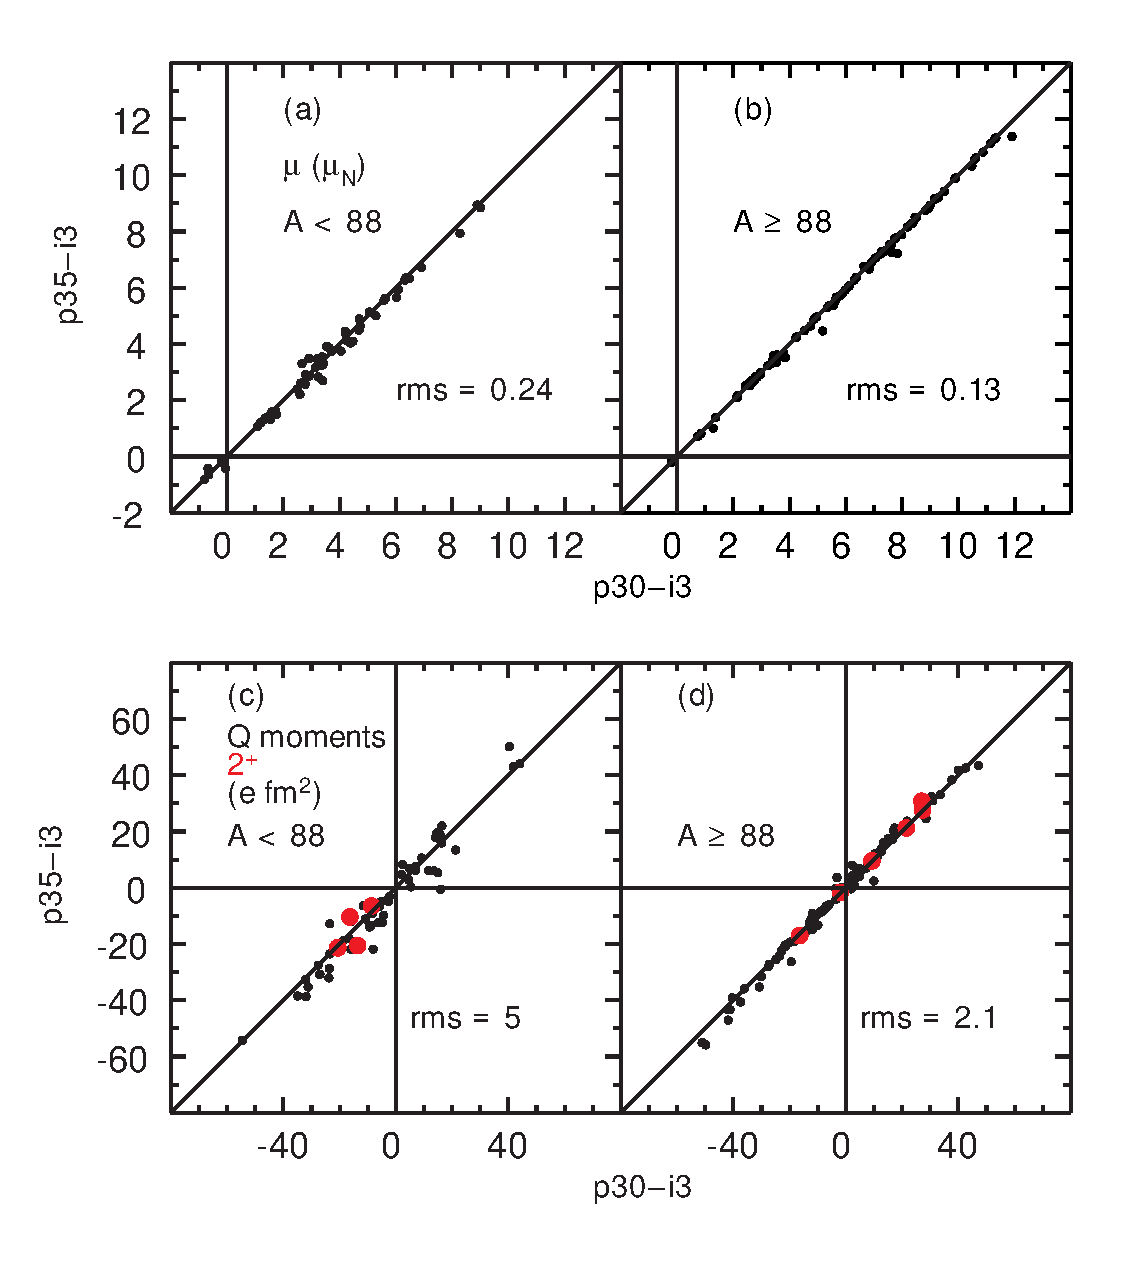
\includegraphics[scale=0.40]{mi3.eps}
\caption{Comparison of  moments obtained with the
p30-i3 and p35-i3 Hamiltonians.
}
\label{ (1) }
\end{figure}

\begin{figure}
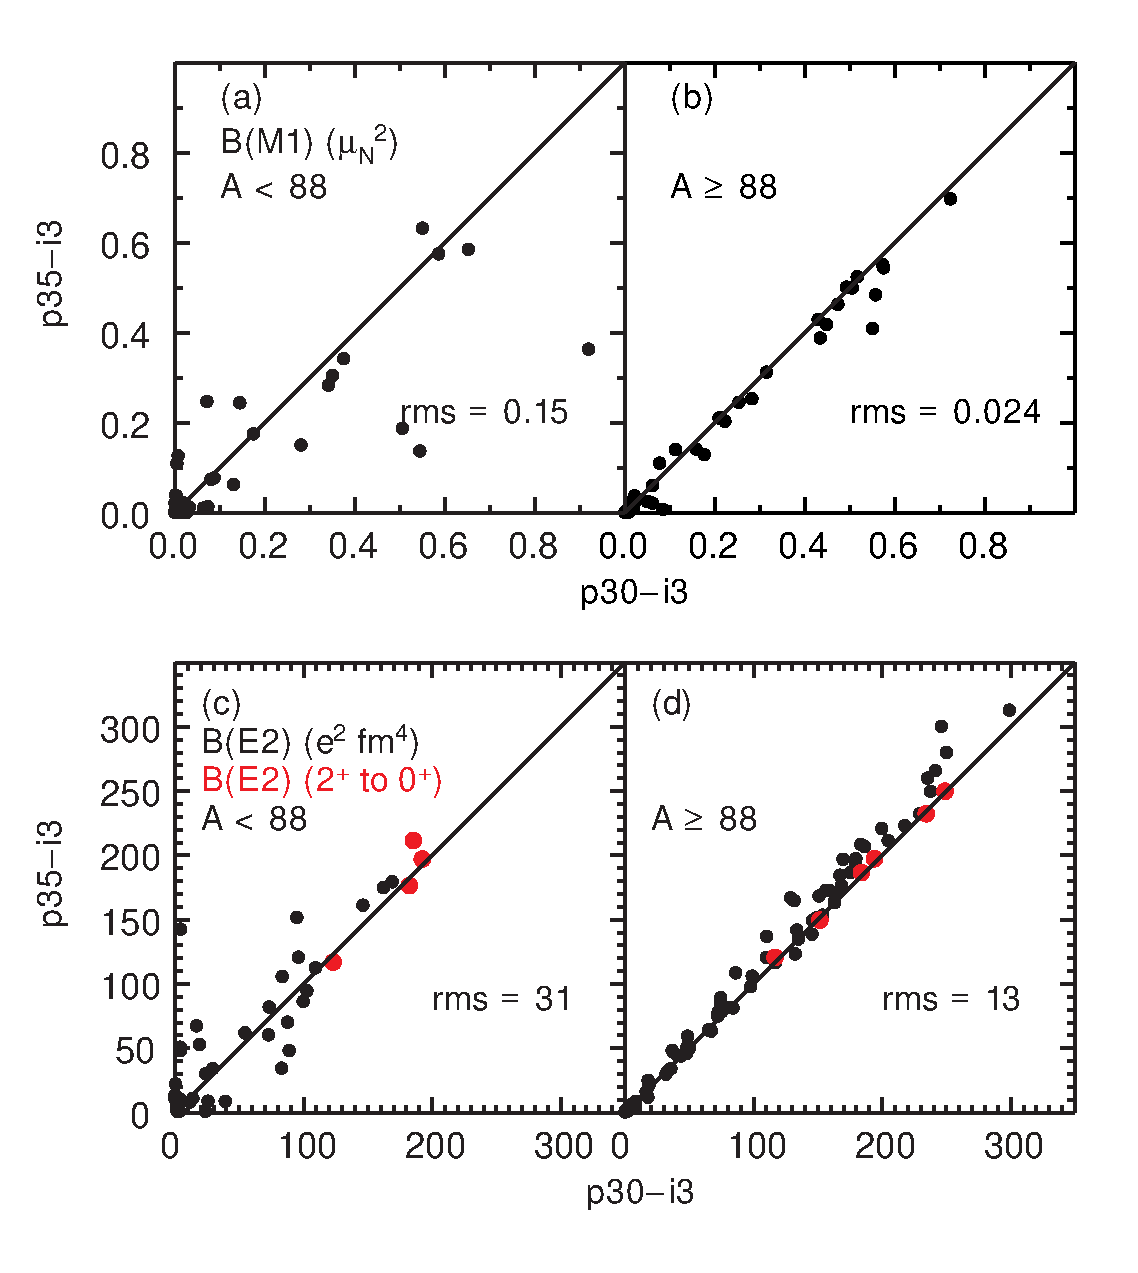
\includegraphics[scale=0.40]{bi3.eps}
\caption{Comparison of B(M1) and B(E2) values obtained with the
p30-i3 and p35-i3 Hamiltonians.
}
\label{ (2) }
\end{figure}




\begin{figure}
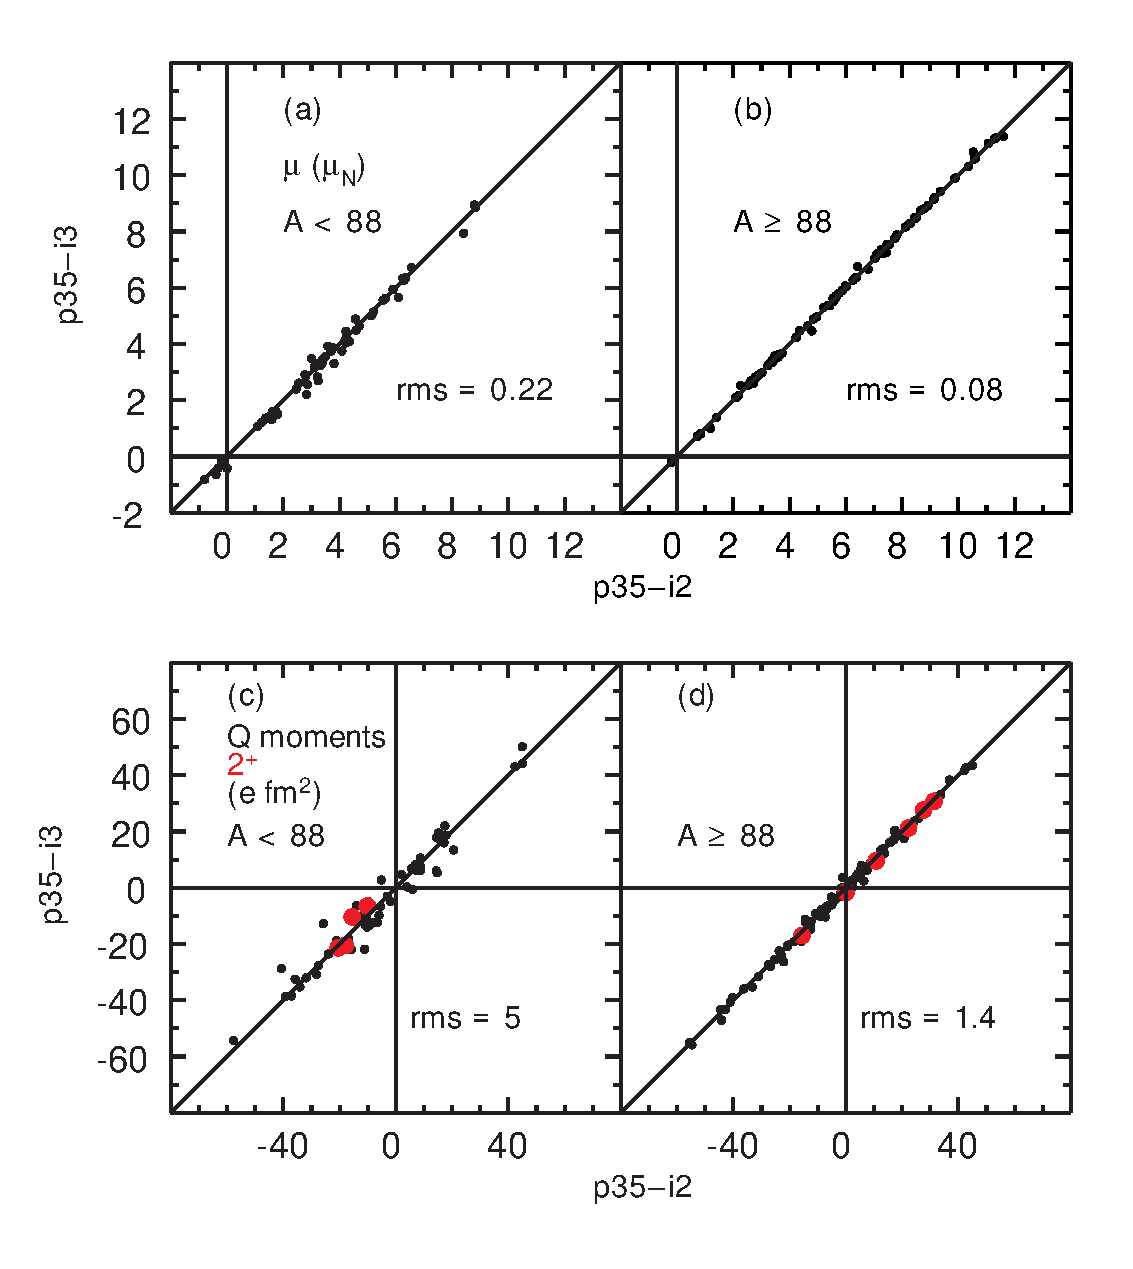
\includegraphics[scale=0.40]{m35.eps}
\caption{Comparison of  moments obtained with the
p35-i2 and p35-i3 Hamiltonians.
}
\label{ (3) }
\end{figure}

\begin{figure}
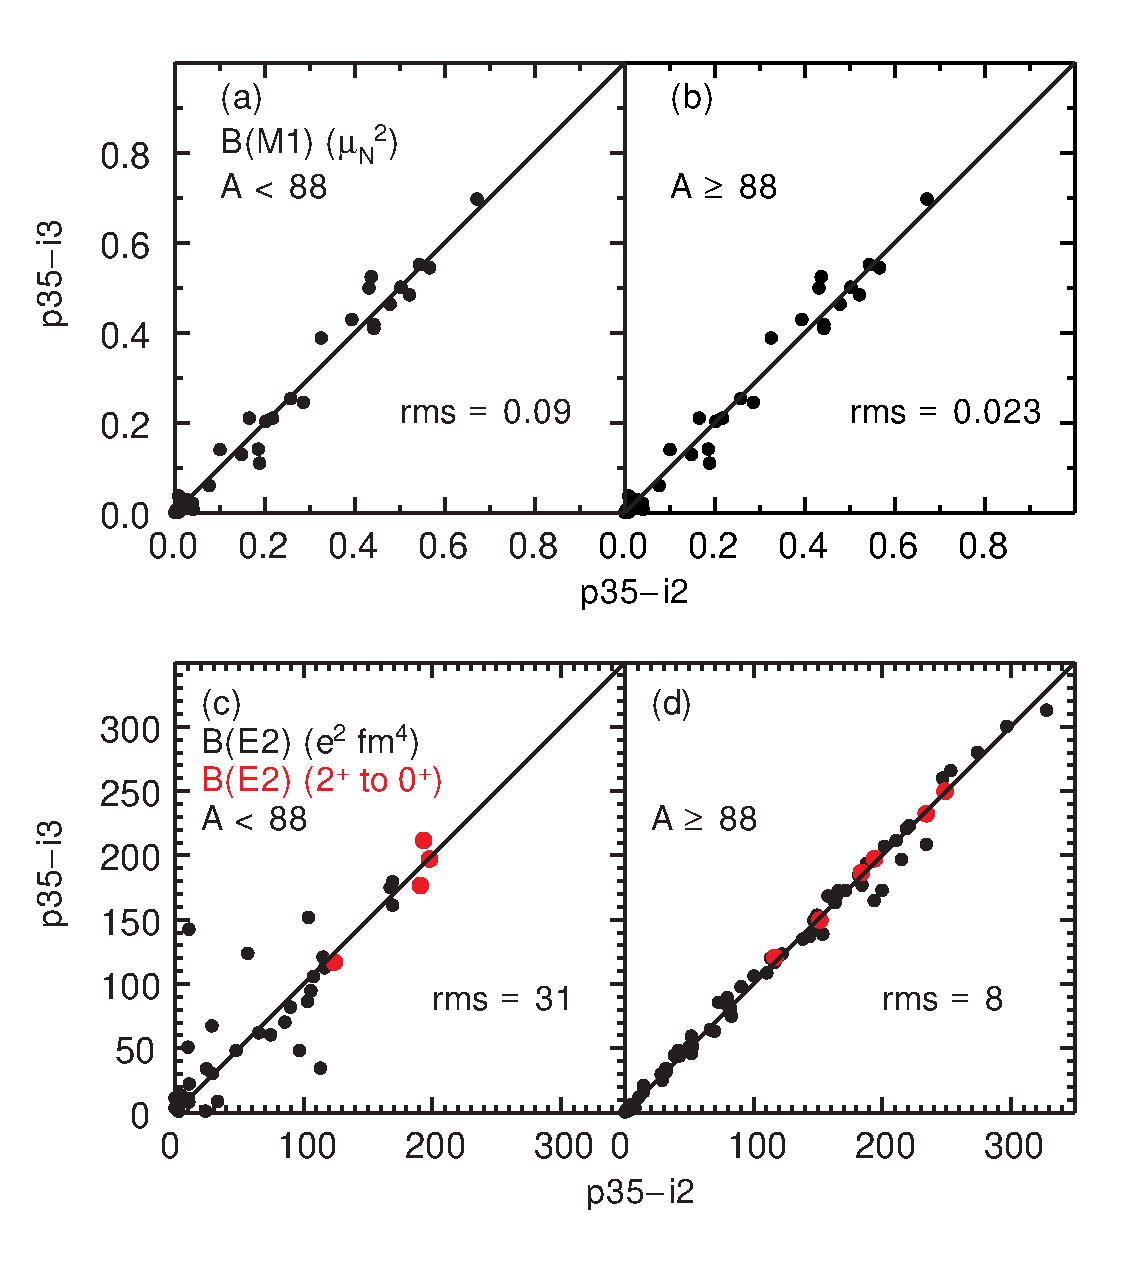
\includegraphics[scale=0.40]{b35.eps}
\caption{Comparison of B(M1) and B(E2) values obtained with the
p35-i2 and p35-i3 Hamiltonians.
}
\label{ (4) }
\end{figure}



\begin{figure}
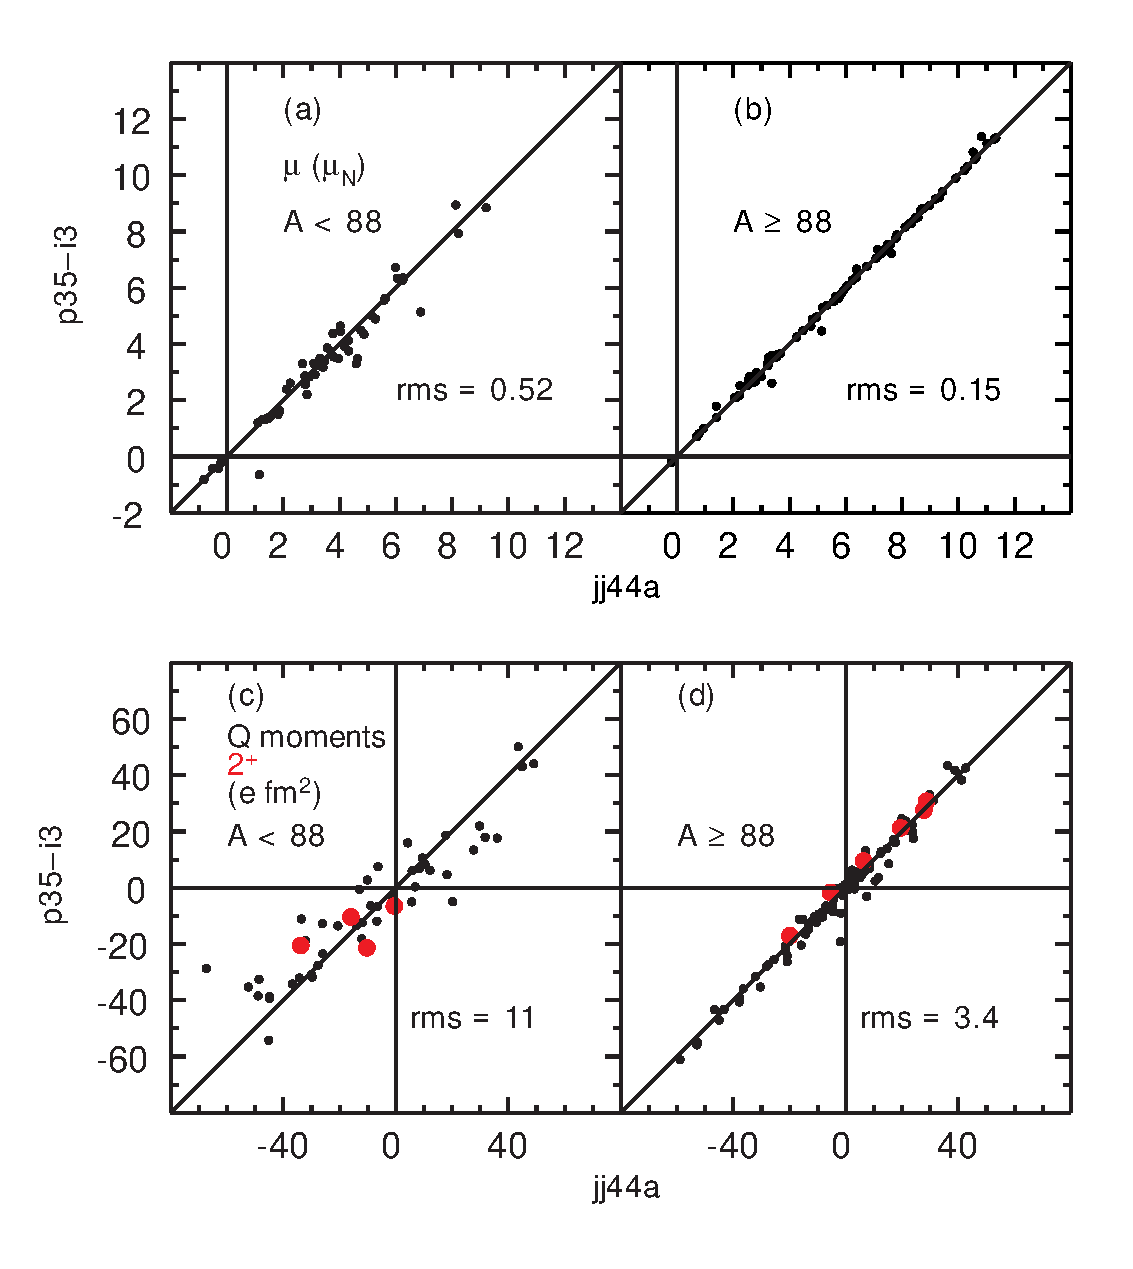
\includegraphics[scale=0.40]{ma.eps}
\caption{Comparison of  moments obtained with the
jj44a and p35-i3 Hamiltonians.
}
\label{ (5) }
\end{figure}

\begin{figure}
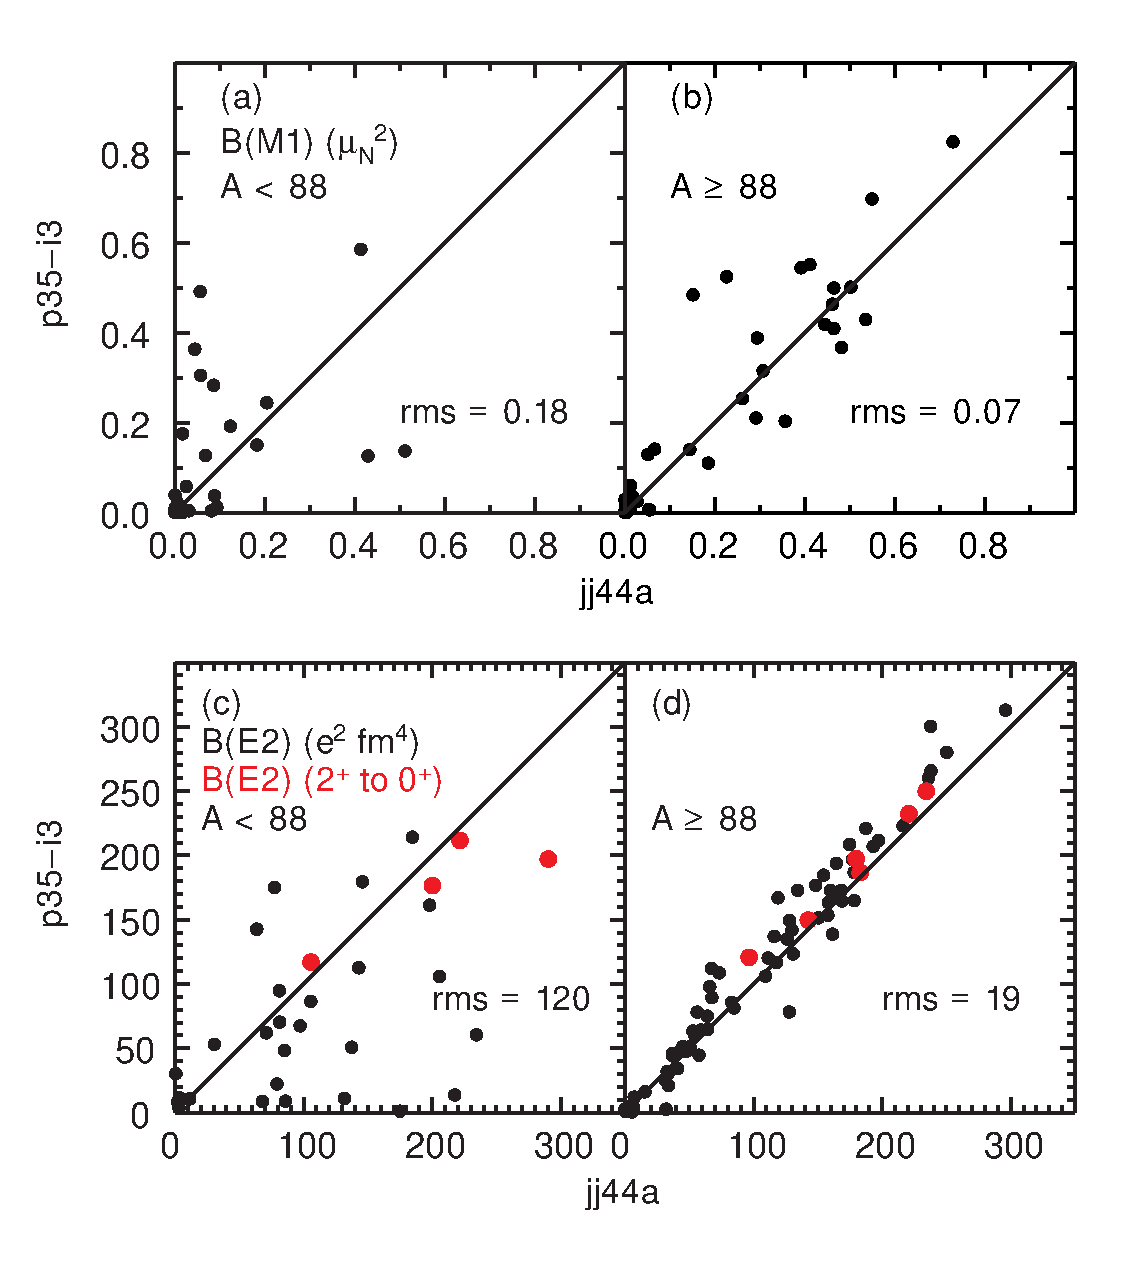
\includegraphics[scale=0.40]{ba.eps}
\caption{Comparison of B(M1) and B(E2) values obtained with the
jj44a and p35-i3 Hamiltonians.
}
\label{ (6) }
\end{figure}



\begin{figure}
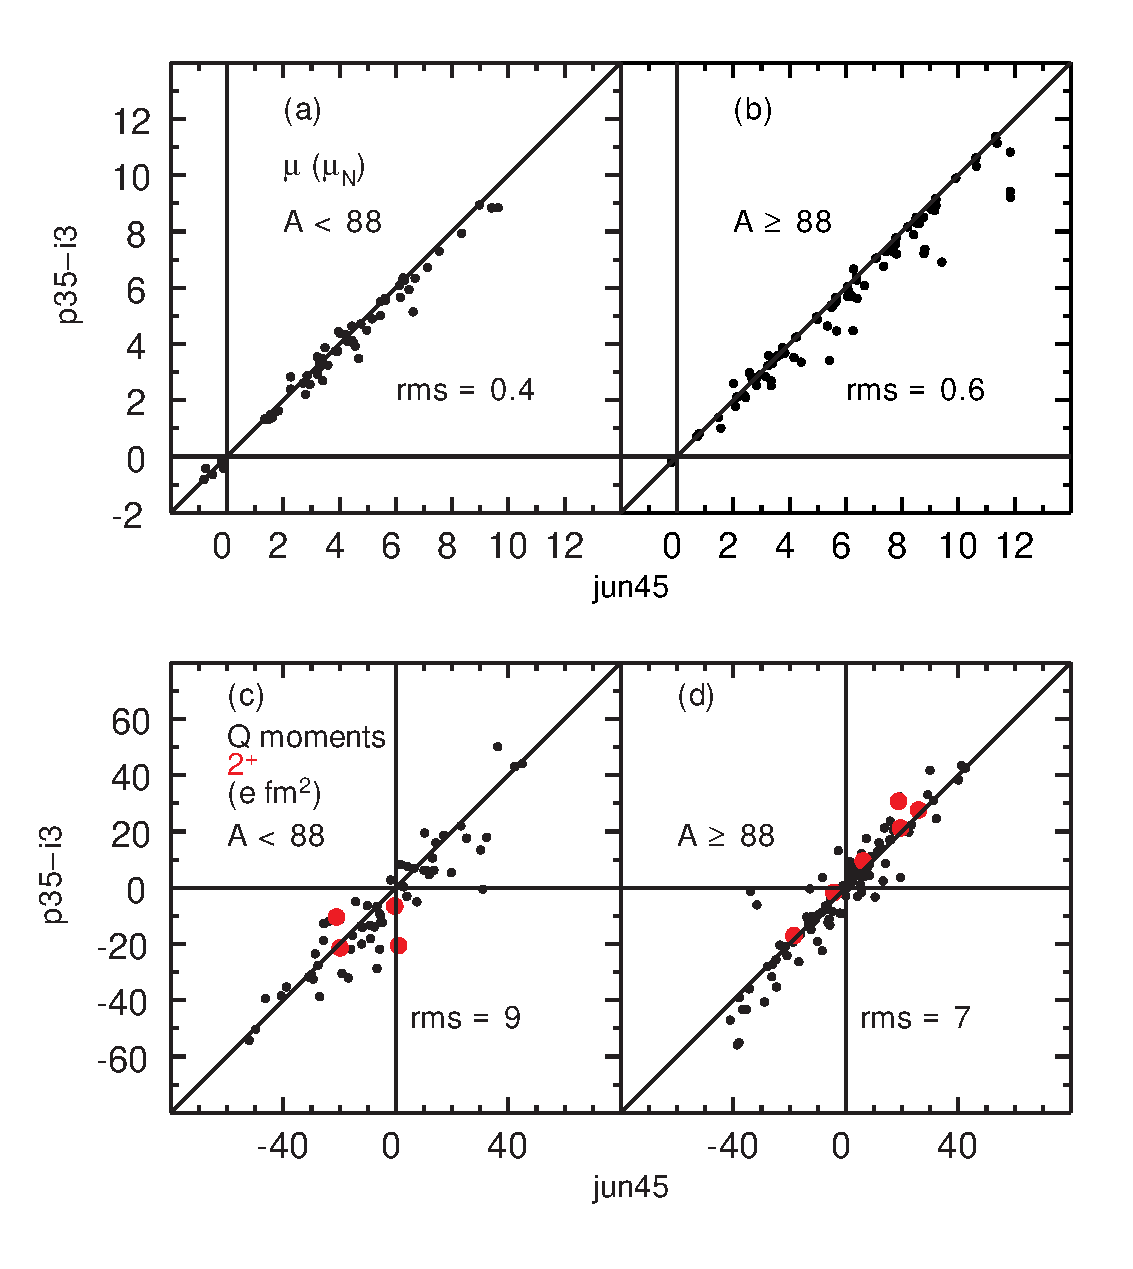
\includegraphics[scale=0.40]{mh.eps}
\caption{Comparison of  moments obtained with the
jun45 and p35-i3 Hamiltonians.
}
\label{ (7) }
\end{figure}

\begin{figure}
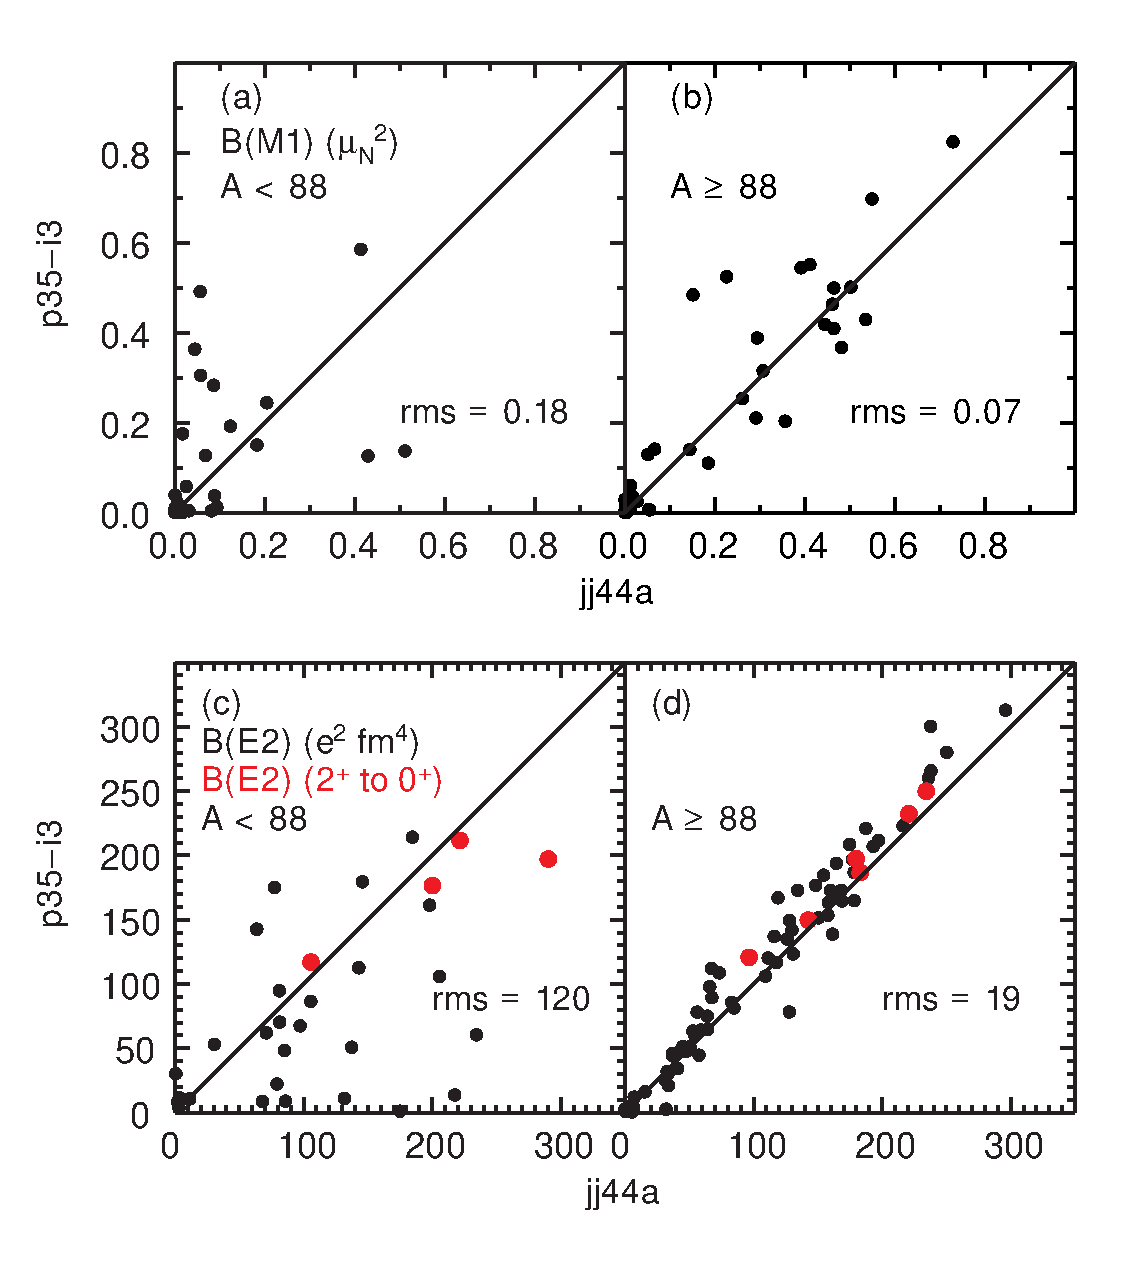
\includegraphics[scale=0.40]{ba.eps}
\caption{Comparison of B(M1) and B(E2) values obtained with the
jun45 and p35-i3 Hamiltonians.
}
\label{ (8) }
\end{figure}




\begin{figure}
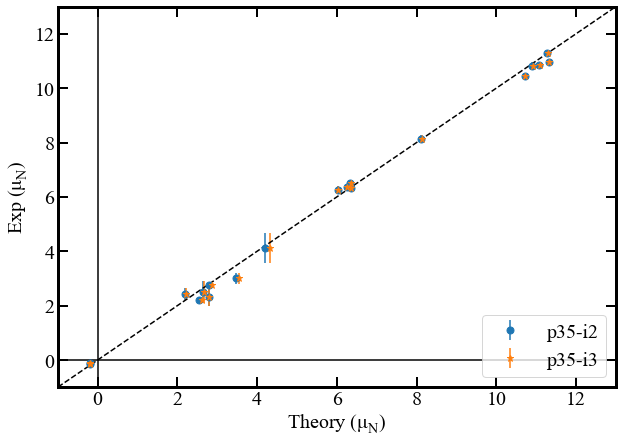
\includegraphics[scale=0.35]{dipoles.png}
\caption{
}
\label{ (9) }
\end{figure}

\begin{figure}
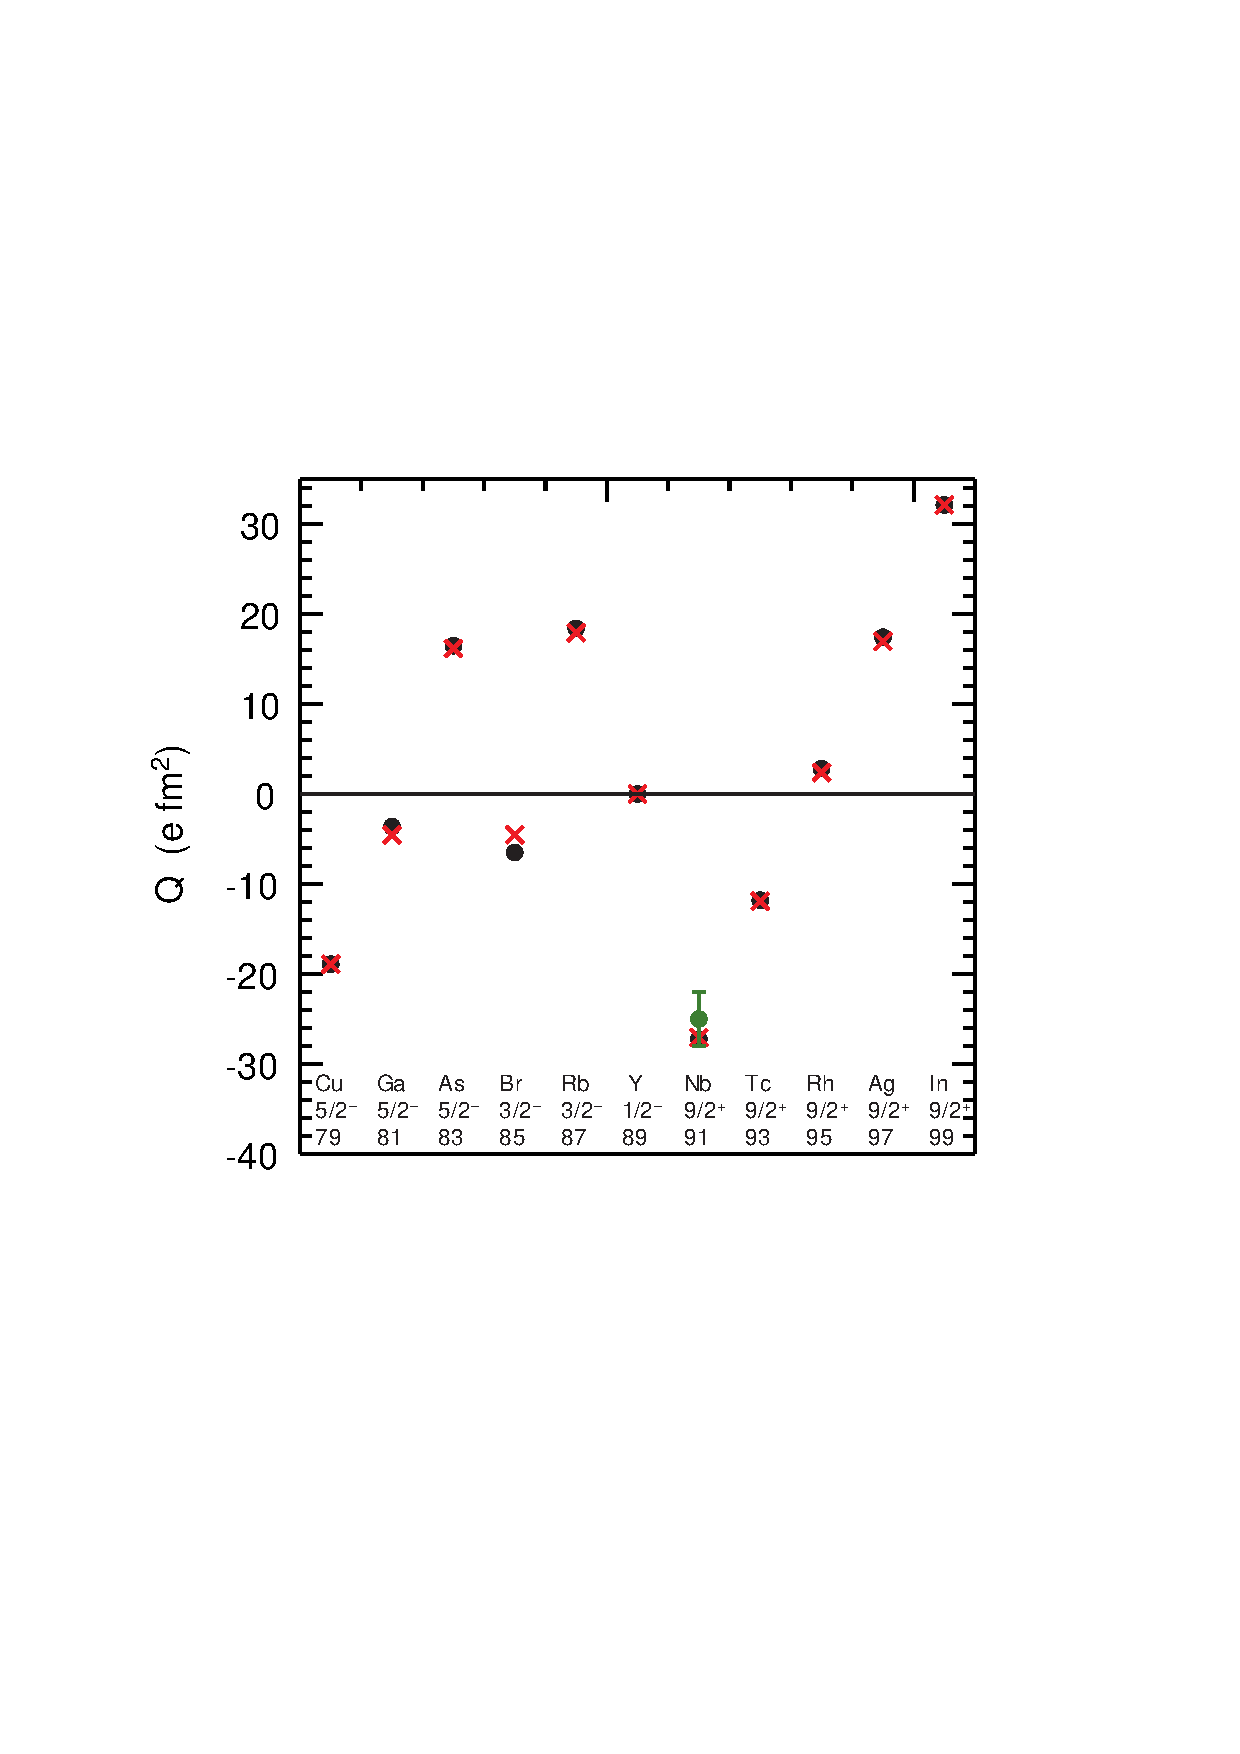
\includegraphics[scale=0.35]{qm.png}
\caption{
}
\label{ (10) }
\end{figure}

\begin{figure}
\includegraphics[scale=0.35]{qmfree.png}
\caption{
}
\label{ (11) }
\end{figure}

\begin{figure}
\includegraphics[scale=0.30]{muq.png}
\caption{
}
\label{ (12) }
\end{figure}

\begin{figure}
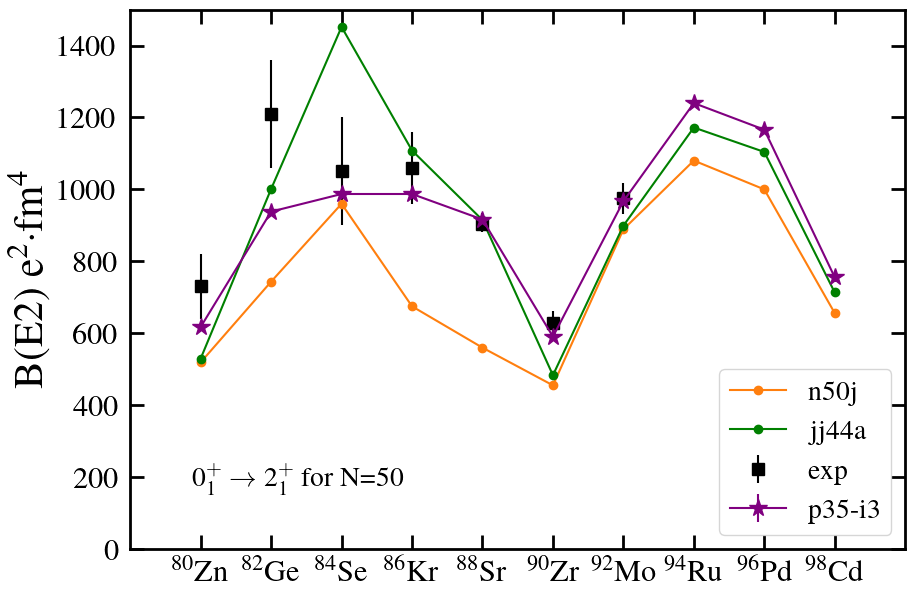
\includegraphics[scale=0.35]{be02.png}
\caption{
}
\label{ (13) }
\end{figure}

\begin{figure}
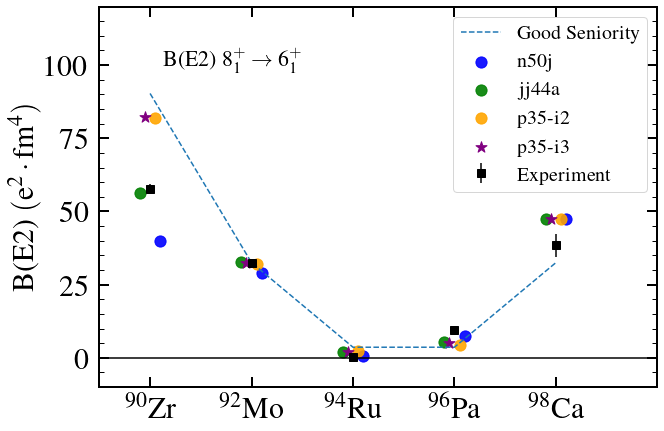
\includegraphics[scale=0.35]{be86.png}
\caption{
}
\label{ (14) }
\end{figure}














\section{Comparison between theory and experiment}

Jordan will add his figures and discussion here




\section{Configuration with $  j^{n}  $}

Will modify this section




For states with good seniority the $  B(E2)  $
between $  j^{n}  $ configurations with $  \nu   $=2 is given by \cite{bh22}
$$
B(E2)(j^{n},J_{i} \rightarrow J_{f})  =
\left[\frac{2j+1-2n}{2j+1-2\nu }\right]^{2} B(E2)(j^{2},J_{i} \rightarrow J_{f}).
$$
For example, for $  j=9/2  $ and $  n=4  $ (or $  n=6  $)
$$
B(E2,j^{4},\nu =2) = (1/9) B(E2,j^{2},\nu =2).
$$



\section{Acknowledgements}


We acknowledge support from the National Science Foundation grant PHY-2110365.



\begin{thebibliography}{9}
\bibitem{talmi60} 
 I. Talmi and I. Unna, Nucl. Phys. {\bf 19}, 225 (1960). 
\bibitem{cohen64} 
S. Cohen, R. D. Lawson, M. H. Macfarlane, and M. 
Soga, Phys. Lett. {\bf 10}, 195 (1964). 
\bibitem{aurbach65} 
 N. Auerbach and I. Talmi, Nucl. Phys. {\bf 64}, 458 (1965). 
\bibitem{vervier66} 
 J. Vervier, Nucl. Phys. {\bf 75}, 17 (1966). 
\bibitem{ball72} 
J. B. Ball, J. B.McGrory, and J. S. Larsen, Phys. 
Lett. {\bf 41B}, 581 (1972). 
\bibitem{gloeckner73} 
D. H. Gloeckner and F. J. D. Serduke, Nucl. Phys . 
 {\bf A220}, 4 (1973). 
\bibitem{blomqvist85} 
 J. Blomqvist and L. Rysdtrom, Phys. Scr. {\bf 31}, 31 (1985). 
\bibitem{jun45} 
M. Honma, T. Otsuka, T. Mizusaki, and M. Hjorth-Je 
nsen, Phys. Rev. C {\bf 80}, 064323 (2009). 
\bibitem{jw88} 
 X. Ji and B. H. Wildenthal, Phys. Rev. C {\bf 37}, 1256 (1988). 
\bibitem{jj44a} 
A. F. Lisetskiy, B. A. Brown, M. Horoi and H. Grawe, 
 Phys. Rev. C {\bf 70}, 044314 (2004). 
\bibitem{Yuan24} 
 Q. Yuan and B. S. Hu, Phys. Lett. B {\bf 858}, 139018 (2024). 
\bibitem{p35i3} 
J. A. Purcell, B. A. Brown, B. C. He, S. R. Strober 
g, and W. B. Walters, 
     Phys. Rev. C {\bf 111}, 044313 (2025). 
\bibitem{Heb2011} 
K. Hebeler, S. K. Bogner, R. J. Furnstahl, A. Nogga, 
and A. Schwenk Phys. Rev. C {\bf 83}, 031301(R) (2011) 
\bibitem{sr19} 
S. R. Stroberg, H. Hergert, S. K. Bogner, and J. D. 
 Holt, Annu. Rev. Nucl. Part. Sci. 2019. {\bf 69}, 307 (2019). 
\bibitem{He24} 
B. C. He and S. R. Stroberg, Phys. Rev. C {\bf 110}, 
044317 (2024). 
\bibitem{nushellx} 
B. A. Brown and W. D. M. Rae, Nuclear Data Sheet 
s {\bf 120}, 115 (2014). 
\bibitem{jw88em} 
 X. Ji and B. H. Wildenthal, Phys. Rev. C {\bf 38}, 2849 (1988). 
\bibitem{skx} 
 B. A. Brown, Phys. Rev. C {\bf 58}, 220 (1998). 
\bibitem{ga81} 
 V. Paziy {\it et al.}, Phys. Rev. C {\bf 102}, 014329 (2020). 
\bibitem{bh22} 
 B. Maheshwari and K. Nomura, Symmetry {\bf 14}, 2680 (2022). 
\end{thebibliography}

\end{document}

